\begin{frame}{Decision Trees: Nền tảng của Random Forest}
    \begin{columns}[T]
        \begin{column}{0.55\textwidth}
                Decision Tree học bằng cách chia dữ liệu theo các điều kiện trên đặc trưng:
                \begin{itemize}
                    \item Mỗi nút là một phép thử
                    \item Chọn split tốt nhất theo Gini/Entropy
                    \item Lặp lại đến khi nút đủ ``thuần'' hoặc đạt điều kiện dừng
                \end{itemize}

        \end{column}

        \begin{column}{0.4\textwidth}
                \centering
                % \fbox{\parbox[c][2.9cm][c]{0.9\linewidth}{\centering Ch\`en \h`inh minh h\d{o}a Decision Tree v\`ao \^o n\`ay}}
                % Sau khi co anh, co the thay bang:
                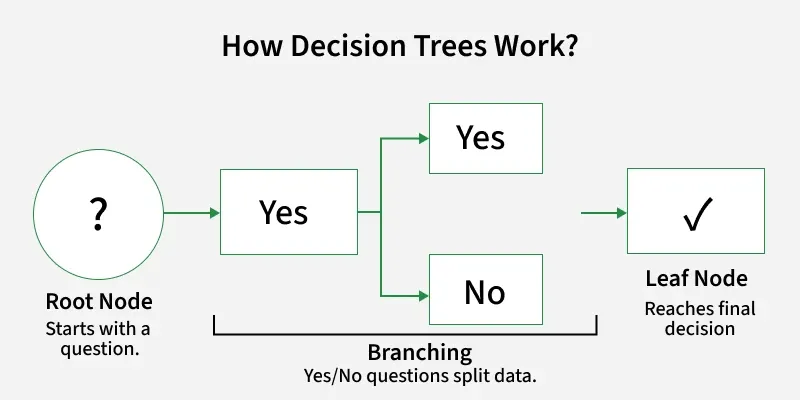
\includegraphics[width=0.95\linewidth]{img/how_decision_trees_work_.png}
        \end{column}
    \end{columns}

                \begin{alertblock}{Vấn đề chính}
                \textbf{Decision Trees dễ overfitting}!
                \begin{itemize}
                    \item Một cây học từ một con đường quyết định duy nhất
                    \item Không dự báo tốt trên dữ liệu mới
                    \item Phương pháp khắc phục: \textbf{Random Forest}
                \end{itemize}
            \end{alertblock}
\end{frame}

\begin{frame}[shrink=8]{Random Forest: Giảm Overfitting}

                Random Forest là một bộ ước lượng tổng quát được phát triển bởi Leo Breiman để giảm overfitting:
                \begin{itemize}
                    \item Xây dựng \textbf{nhiều cây quyết định}
                    \item Trên các \textbf{mẫu con khác nhau} của dữ liệu
                    \item Sử dụng \textbf{trung bình hóa} để cải thiện độ chính xác
                \end{itemize}

            \begin{block}{Giảm Overfitting: Quy trình}
                \begin{itemize}
                    \item Tạo $n\_estimators$ cây quyết định
                    \item Mỗi cây học trên bootstrap sample (lấy mẫu có hoàn lại)
                    \item Mỗi nút chỉ xét tập con ngẫu nhiên của đặc trưng
                    \item Dự đoán cuối: vote (phân loại) hoặc trung bình (hồi quy)
                \end{itemize}
            \end{block}
\end{frame}

\begin{frame}[shrink=10]{Random Forest vs Extra Trees: Sự khác biệt}
    \centering
    \begin{tabular}{p{0.22\linewidth} p{0.35\linewidth} p{0.35\linewidth}}
        \toprule
        \textbf{Tiêu chí} & \textbf{Random Forest} & \textbf{Extra Trees} \\
        \midrule
        \textbf{Bootstrap sampling} & Có (lấy mẫu có hoàn lại) & Không (lấy mẫu có hoàn lại) \\
        \textbf{Cách chọn split} & Chọn best split ở mỗi nút & Chọn split ngẫu nhiên ở mỗi nút \\
        \textbf{Phương sai} & Cao hơn & Thấp hơn \\
        \textbf{Bias} & Thấp hơn & Cao hơn \\
        \textbf{Tốc độ} & Chậm hơn (phải tìm best split) & Nhanh hơn (random split) \\
        \bottomrule
    \end{tabular}
    \vspace{0.2cm}
    
    \begin{alertblock}{Lưu ý}
        \textbf{ExtraTrees} được gọi là ``Extremely Randomized Trees''. Nó dùng random splits thay vì best splits để giảm phương sai, nhưng tăng bias.
    \end{alertblock}
\end{frame}

\begin{frame}[shrink=10]{Random Forest: Đánh giá}
    \begin{columns}[T]
        \begin{column}{0.48\textwidth}
            \textbf{Ưu điểm:}
            \begin{itemize}
                \item Giảm overfitting tốt hơn cây đơn lẻ
                \item Ổn định nhờ trung bình hóa nhiều cây
                \item Ít cần chuẩn hóa dữ liệu đầu vào
            \end{itemize}
        \end{column}
        \begin{column}{0.48\textwidth}
            \textbf{Nhược điểm:}
            \begin{itemize}
                \item Khó diễn giải hơn Decision Tree
                \item Chi phí suy luận tăng khi số cây lớn
                \item Có thể kém hơn SVM ở một số bài toán biên rõ
            \end{itemize}
        \end{column}
    \end{columns}

    \begin{alertblock}{Kết quả mẫu (Breast Cancer)}
        Cấu hình: \texttt{n\_estimators=100}, train/test split $50\%$:
        \begin{itemize}
            \item \textbf{bAcc}: 0.93
            \item \textbf{AUC}: 0.98
            \item So với SVM (bAcc=0.97, AUC=0.99): thấp hơn nhẹ nhưng dễ dùng
        \end{itemize}
    \end{alertblock}

    \hfill{\scriptsize \cite{duchesnay2021statsml}}
\end{frame}
